%============================================================
\section{Nombre: Raíz del diablo.}\label{hab.RaizDia}
\subsection{Descripción}
Onda roja que produce confusión en el jugador por un periodo de tiempo determinado al hacer contacto con él. La onda incrementara su diámetro hasta alcanzar un diámetro máximo, una vez alcanzado ese diámetro máximo desaparecerá. Bajo el estado de confusión los controles de la GUI no responderán de manera efectiva intercambiando funcionalidad, es decir el botón de saltar moverá al personaje a la derecha, el botón de disparo será para saltar, el botón de mover hacia la izquierda será para disparar y el botón de mover hacia derecha moverá al personaje a la izquierda. 
\subsection{Portador}
Tlazoltéotl (ver apartado \ref{per:tlazolteotl}).
\subsection{Esquema}
			Ver figura \ref{fig:raiz}.
			\begin{figure}
				\centering
				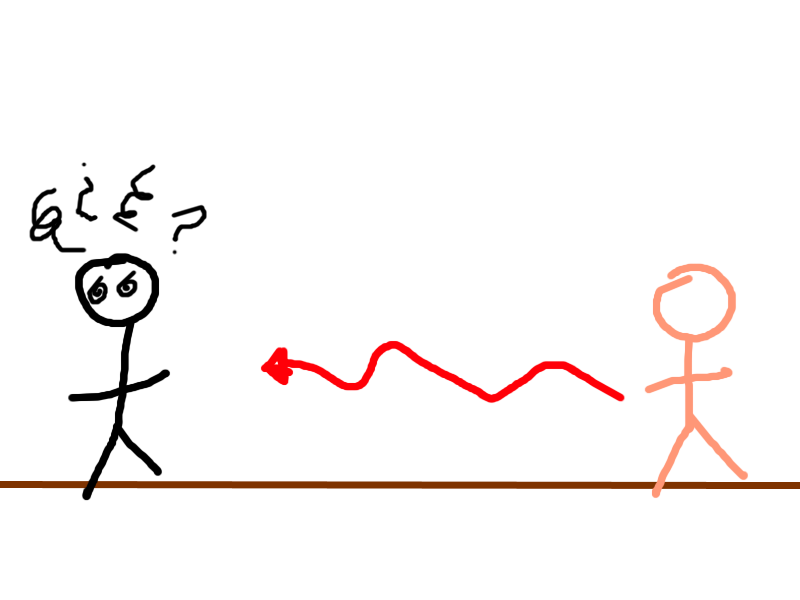
\includegraphics[height=0.2 \textheight]{Imagenes/raiz}
				\caption{Raíz del diablo.}
				\label{fig:raiz}
			\end{figure}